\documentclass[10pt,a4paper]{article}
\usepackage[UTF8,fontset = windows]{ctex}
\setCJKmainfont[BoldFont=黑体,ItalicFont=楷体]{华文中宋}
\usepackage{amssymb,amsmath,amsfonts,amsthm,mathrsfs,dsfont,graphicx}
\usepackage{ifthen,indentfirst,enumerate,color,titletoc}
\usepackage{tikz}
\usetikzlibrary{arrows,calc,intersections}
\usepackage[bf,small,indentafter,pagestyles]{titlesec}
\usepackage[top=1in, bottom=1in,left=0.8in,right=0.8in]{geometry}
\renewcommand{\baselinestretch}{1.65}
\newtheorem{defi}{定义~}
\newtheorem{eg}{例~}
\newtheorem{ex}{~}
\newtheorem{rem}{注~}
\newtheorem{thm}{定理~}
\newtheorem{coro}{推论~}
\newtheorem{axiom}{公理~}
\newtheorem{prop}{性质~}

\newcommand{\blank}[1]{\underline{\hbox to #1pt{}}}
\newcommand{\bracket}[1]{(\hbox to #1pt{})}

\newcommand{\onech}[4]{\par\begin{tabular}{p{.9\textwidth}}
A.~#1\\
B.~#2\\
C.~#3\\
D.~#4
\end{tabular}}

\newcommand{\twoch}[4]{\par\begin{tabular}{p{.46\textwidth}p{.46\textwidth}}
A.~#1& B.~#2\\
C.~#3& D.~#4
\end{tabular}}

\newcommand{\vartwoch}[4]{\par\begin{tabular}{p{.46\textwidth}p{.46\textwidth}}
(1)~#1& (2)~#2\\
(3)~#3& (4)~#4
\end{tabular}}


\newcommand{\fourch}[4]{\par\begin{tabular}{p{.23\textwidth}p{.23\textwidth}p{.23\textwidth}p{.23\textwidth}}
A.~#1 &B.~#2& C.~#3& D.~#4
\end{tabular}}

\newcommand{\varfourch}[4]{\par\begin{tabular}{p{.23\textwidth}p{.23\textwidth}p{.23\textwidth}p{.23\textwidth}}
(1)~#1 &(2)~#2& (3)~#3& (4)~#4
\end{tabular}}
    

\begin{document}

{\bf 2021年秋考}

\begin{enumerate}[1.]
\item 已知$z_1=1+\mathrm{i}$, $z_2=2+3\mathrm{i}$($\mathrm{i}$是虚数单位), 则$z_1+z_2=$\blank{50}.
\item 已知$A=\{x|2x\le 1\}$, $B=\{-1,0,1\}$, 则$A\cap B=$\blank{50}.
\item 已知圆$x^2+y^2-2x-4y=0$, 则该圆的圆心坐标为\blank{50}.
\item 如图, 正方形$ABCD$的边长为$3$, 则$\overrightarrow{AB}\cdot \overrightarrow{AC}=$\blank{50}.
\begin{center}
    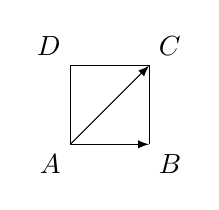
\begin{tikzpicture}[>=latex]
        \draw (0,0) -- (0,1) node [above left] {$D$}  -- (1,1) -- (1,0);
        \draw [->] (0,0) node [below left] {$A$} -- (1,1) node [above right] {$C$};
        \draw [->] (0,0) -- (1,0) node [below right] {$B$};
    \end{tikzpicture}
\end{center}
\item 已知$f(x)=\dfrac3x+2$, 则$f^{-1}(1)=$\blank{50}.
\item 已知二项式$(x+a)^5$展开式中, $x^2$项的系数为$80$, 则$a=$\blank{50}.
\item 已知实数$x,y$满足$\begin{cases} x\le 3,  \\ 2x-y-2 \ge 0,  \\ 3x+y-8 \ge 0,  \end{cases}$ 则$z=x-y$的最大值为\blank{50}.
\item 已知无穷等比数列$\{a_n\}$和$\{b_n\}$, 满足$a_1=3$, $b_n=a_{2n}$, $a_n$的各项和为$9$, 则数列$\{b_n\}$的各项和为\blank{50}.
\item 已知圆柱的底面半径为$1$, 高为$2$, AB为上底面圆的一条直径, $C$为下底面圆周上的一个动点, 则$\triangle ABC$的面积的取值范围为\blank{50}.
\item 已知花博会有四个不同的场馆A、B、C、D, 甲、乙两人每人选$2$个去参观, 则他们的选择中, 恰有一个场馆相同的概率为\blank{50}.
\item 已知抛物线:$y^2=2px \ (p>0)$, 若第一象限的$A,B$两点在抛物线上, 焦点为$F$, $|AF|=2$, $|BF|=4$, $|AB|=3$, 则直线$AB$的斜率为\blank{50}.
\item 已知$a_i\in \mathbf{N}^* \ (i=1,2,\cdots,9)$, 若对任意的$k\in \mathbf{N}^* \ (2\le k\le 8)$, $a_k=a_{k-1}+1$或$a_k=a_{k+1}-1$中有且仅有一个成立, 且$a_1=6$, $a_9=9$, 则$a_1+a_2+\cdots+a_9$的最小值为\blank{50}.
\item 下列函数中, 既是奇函数又是减函数的是\bracket{20}.
\fourch{$y=-3x$}{$y=x^3$}{$y=\log_3^x$}{$y=3^x$}
\item 已知参数方程$\begin{cases} x=3t-4t^3, \\ y=2t\sqrt{1-t^2}, \end{cases} (t\in [-1,1])$, 下列选项的图中, 该参数方程对应的曲线为\bracket{20}.
\fourch{
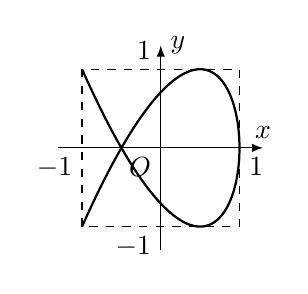
\begin{tikzpicture}[>=latex]
    \draw [->] (-1.3,0) -- (1.3,0) node [above] {$x$};
    \draw [->] (0,-1.3) -- (0,1.3) node [right] {$y$};
    \draw (0,0) node [below left] {$O$};
    \draw [dashed] (-1,-1) -- (-1,1) -- (1,1) -- (1,-1) -- cycle;
    \draw (1,0) node [below right] {$1$} (-1,0) node [below left] {$-1$} (0,1) node [above left] {$1$} (0,-1) node [below left] {$-1$};
    \draw [thick, domain = 0:360, samples = 200] plot ({cos(2*\x)},{sin(3*\x)}); 
\end{tikzpicture}    
}{
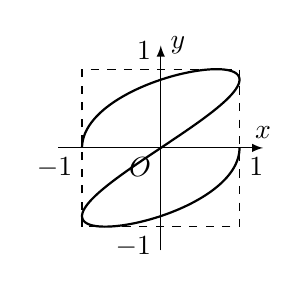
\begin{tikzpicture}[>=latex]
    \draw [->] (-1.3,0) -- (1.3,0) node [above] {$x$};
    \draw [->] (0,-1.3) -- (0,1.3) node [right] {$y$};
    \draw (0,0) node [below left] {$O$};
    \draw [dashed] (-1,-1) -- (-1,1) -- (1,1) -- (1,-1) -- cycle;
    \draw (1,0) node [below right] {$1$} (-1,0) node [below left] {$-1$} (0,1) node [above left] {$1$} (0,-1) node [below left] {$-1$};
    \draw [thick, domain = 0:180, samples = 200] plot ({-cos(3*\x)},{sin(2*\x)}); 
\end{tikzpicture} 
}{
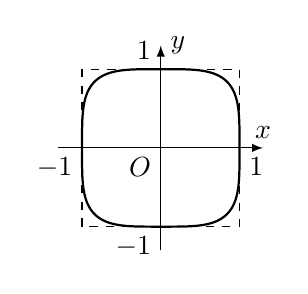
\begin{tikzpicture}[>=latex]
    \draw [->] (-1.3,0) -- (1.3,0) node [above] {$x$};
    \draw [->] (0,-1.3) -- (0,1.3) node [right] {$y$};
    \draw (0,0) node [below left] {$O$};
    \draw [dashed] (-1,-1) -- (-1,1) -- (1,1) -- (1,-1) -- cycle;
    \draw (1,0) node [below right] {$1$} (-1,0) node [below left] {$-1$} (0,1) node [above left] {$1$} (0,-1) node [below left] {$-1$};
    \draw [thick, domain = 0:90, samples = 200] plot ({sqrt(cos(\x))},{sqrt(sin(\x))});
    \draw [thick, domain = 0:90, samples = 200] plot ({-sqrt(cos(\x))},{sqrt(sin(\x))});
    \draw [thick, domain = 0:90, samples = 200] plot ({sqrt(cos(\x))},{-sqrt(sin(\x))}); 
    \draw [thick, domain = 0:90, samples = 200] plot ({-sqrt(cos(\x))},{-sqrt(sin(\x))});
\end{tikzpicture} 
}{
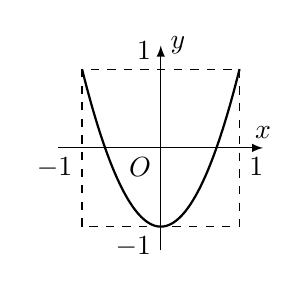
\begin{tikzpicture}[>=latex]
    \draw [->] (-1.3,0) -- (1.3,0) node [above] {$x$};
    \draw [->] (0,-1.3) -- (0,1.3) node [right] {$y$};
    \draw (0,0) node [below left] {$O$};
    \draw [dashed] (-1,-1) -- (-1,1) -- (1,1) -- (1,-1) -- cycle;
    \draw (1,0) node [below right] {$1$} (-1,0) node [below left] {$-1$} (0,1) node [above left] {$1$} (0,-1) node [below left] {$-1$};
    \draw [thick, domain = 0:360, samples = 200] plot ({sin(\x)},{-cos(2*\x)});
\end{tikzpicture}     
}
\item 已知$f(x)=3\sin x+2$, 对任意的$x_1\in [0,\dfrac{\pi}2]$, 都存在$x_2\in [0,\dfrac{\pi}2]$, 使得$f({x_1})+2f(x_2+\theta)=3$成立, 则在下列选项中$\theta$可能的值为\bracket{20}.
\fourch{$\dfrac{3\pi}5$}{$\dfrac{4\pi}5$}{$\dfrac{6\pi}5$}{$\dfrac{7\pi}5$}
\item 已知两两不等的实数$x_1,y_1,x_2,y_2,x_3,y_3$同时满足: \textcircled{1} $x_1<y_1$, $x_2<y_2$, $x_3<y_3$; \textcircled{2} $x_1+y_1=x_2+y_2=x_3+y_3$; \textcircled{3} $x_1y_1+x_3y_3=2x_2y_2>0$, 则下列选项中恒成立的是\bracket{20}.
\fourch{$2x_2<x_1+x_3$}{$2x_2>x_1+x_3$}{$x_2^2<x_1x_3$}{$x_2^2>x_1x_3$}
\item 如图, 在长方体$ABCD-A_1B_1C_1D_1$中, 已知$AB=BC=2$, $AA_1=3$.\\
(1) 若点$P$是棱$A_1D_1$上的动点, 求三棱锥$C-PAD$的体积;\\
(2) 求直线$AB_1$与平面$ACC_1A_1$的夹角大小.
\begin{center}
    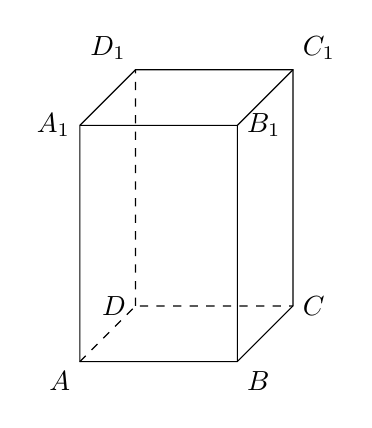
\begin{tikzpicture}
        \draw (0,0) node [below left] {$A$} coordinate (A) --++ (2,0) node [below right] {$B$} coordinate (B) --++ (45:{2/2}) node [right] {$C$} coordinate (C)
        --++ (0,3) node [above right] {$C_1$} coordinate (C1)
        --++ (-2,0) node [above left] {$D_1$} coordinate (D1) --++ (225:{2/2}) node [left] {$A_1$} coordinate (A1) -- cycle;
        \draw (A) ++ (2,3) node [right] {$B_1$} coordinate (B1) -- (B) (B1) --++ (45:{2/2}) (B1) --++ (-2,0);
        \draw [dashed] (A) --++ (45:{2/2}) node [left] {$D$} coordinate (D) --++ (2,0) (D) --++ (0,3);
    \end{tikzpicture}
\end{center}
\item 已知在$\triangle ABC$中,$A,B,C$所对边分别为$a,b,c$, 且$a=3$, $b=2c$.\\
(1) 若$A=\dfrac{2\pi}3$, 求$\triangle ABC$的面积;\\ 
(2) 若$2\sin B-\sin C=1$, 求$\triangle ABC$的周长.
\item 已知某企业今年(2021年)第一季度的营业额为$1.1$亿元, 以后每个季度的营业额比上个季度增加$0.05$亿元, 该企业第一季度的利润为$0.16$亿元, 以后每季度比前一季度增长$4\%$.\\ 
(1) 求2021年起前$20$季度营业额的总和;\\ 
(2) 请问哪一季度的利润首次超过该季度营业额的$18\%$?
\item 已知椭圆$\Gamma:\dfrac{x^2}2+y^2=1$, $F_1, F_2$是其左右焦点, 直线$l$过点$P(m,0) \ (m<-\sqrt2)$, 交椭圆$\Gamma$于$A,B$两点, 且$A,B$都在$x$轴上方, 点$A$在线段$BP$上.\\
(1) 若$B$是上顶点, $|\overrightarrow{BF_1}|=|\overrightarrow{PF_1}|$, 求$m$的值;\\
(2) 若$\overrightarrow{F_1A}\cdot \overrightarrow{F_2A}=\dfrac13$, 且原点$O$到直线$l$的距离为$\dfrac{4\sqrt{15}}{15}$, 求直线$l$的方程;\\
(3) 对于任意点$P$, 是否存在唯一直线$l$, 使得$\overrightarrow{F_1A}\parallel \overrightarrow{F_2B}$成立? 若存在, 求出直线$l$的斜率; 若不存在, 请说明理由.
\item 已知$f(x)$是定义在$\mathbf{R}$上的函数, 若对任意的$x_1,x_2\in \mathbf{R}$, $x_1-x_2\in S$, 均有$f(x_1)-f(x_2)\in S$, 则称$f(x)$是``$S-$关联''的.\\
(1) 判断和证明$f(x)=2x+1$是否是``$[0,+\infty)-$关联''的? 是否是``$[0,1]-$关联''的?\\
(2) 若$f(x)$是``$\{3\}-$关联''的, 且当$x\in [0,3)$时, $f(x)=x^2-2x$, 解不等式$2 \le f(x)\le 3$;\\
(3) 证明: ``$f(x)$是`$\{1\}-$关联'的, 且是`$[0,+\infty)-$关联'的''当且仅当``$f(x)$是`$[1,2]-$关联'的''.







\end{enumerate}

\newpage

{\bf 2020年秋考}

\begin{enumerate}[1.]
\item 已知集合$A=\{1,2,4\}$,$B=\{2,4,5\}$, 则$A\cap B=$\blank{50}.
\item 计算: $\displaystyle\lim_{n\to\infty}\dfrac{n+1}{3n-1}=$\blank{50}.
\item 已知复数$z=1-2 \mathrm{i}$($\mathrm{i}$为虚数单位), 则$|z|=$\blank{50}.
\item 已知函数$f(x)=x^3$, 则其反函数为\blank{50}.
\item 已知$x,y$满足$\begin{cases}x+y-2 \ge 0, \\ x+2y-3 \le 0, \\ y\ge 0, \end{cases}$ 则$z=y-2x$的最大值为\blank{50}.
\item 已知行列式$\begin{vmatrix}1 & a & b  \\ 2 & c & d  \\ 3 & 0 & 0 \end{vmatrix}=6$, 则行列式$\begin{vmatrix} a & b  \\ c & d \end{vmatrix}=$\blank{50}.
\item 已知等差数列$\{a_n\}$的首项$a_1\ne 0$, 且满足$a_1+a_{10}=a_9$, 则$\dfrac{a_1+a_2+\cdots+a_9}{a_{10}}=$\blank{50}.
\item 已知有四个数$1,2,a,b$, 这四个数的中位数为$3$, 平均数为$4$, 则$ab=$\blank{50}.
\item 从$6$个人选$4$个人去值班, 每人值班一天, 第一天安排$1$个人, 第二天安排$1$个人, 第三天安排$2$个人, 则共有\blank{50}种安排情况.
\item 已知椭圆$C:\dfrac{x^2}4+\dfrac{y^2}3=1$, 直线$l$经过椭圆右焦点$F$, 交椭圆$C$于$P,Q$两点(点$P$在第二象限), 若$Q$关于$x$轴对称的点为$Q'$, 且满足$PQ\perp FQ'$, 则直线$l$的方程为\blank{50}.
\item 已知$a\in \mathbf{R}$, 若存在定义域为$\mathbf{R}$的函数$f(x)$同时满足下列两个条件, \textcircled{1} 对任意$x_0\in \mathbf{R}$, $f(x_0)$的值为$x_0$或$x_0^2$; \textcircled{2} 关于$x$的方程$f(x)=a$无实数解; 则$a$的取值范围为\blank{50}.	
\item 已知$\overrightarrow{a_1}, \overrightarrow{a_2}, \overrightarrow{b_1}, \overrightarrow{b_2},\cdots,\overrightarrow{b_k}\ (k\in \mathbf{N}^*)$是平面内两两互不相等的向量, 满足$|\overrightarrow{a_1}-\overrightarrow{a_2}|=1$, 且$|\overrightarrow{a_i}-\overrightarrow{b_j}|\in \{1,2\}$(其中$i=1,2$, $j=1,2,\cdots,k$), 则$k$的最大值为\blank{50}.
\item 下列不等式恒成立的是\bracket{20}.
\fourch{${a^2}+{b^2}\le 2ab$}{${a^2}+{b^2}\ge -2ab$}{$a+b\ge 2 \sqrt{|ab|}$}{$a+b\ge -2 \sqrt{|ab|}$}
\item 已知直线方程$3x+4y+1=0$的一个参数方程可以是\bracket{20}.
\fourch{$\begin{cases}x=1+3t, \\ y=-1+4t \end{cases}$}{$\begin{cases} x=1-4t, \\ y=-1-3t \end{cases}$}{$\begin{cases} x=1-3t, \\ y=-1+4t \end{cases}$}{$\begin{cases} x=1+4t, \\ y=-1-3t \end{cases}$}
\item 在棱长为$10$的正方体$ABCD-A_1B_1C_1D_1$中,$P$为左侧面$ADD_1A_1$上一点, 已知点$P$到$A_1D_1$的距离为$3$, $P$到$AA_1$的距离为$2$, 则过点$P$且与$A_1C$平行的直线相交的正方体的面是\bracket{20}.
\begin{center}
    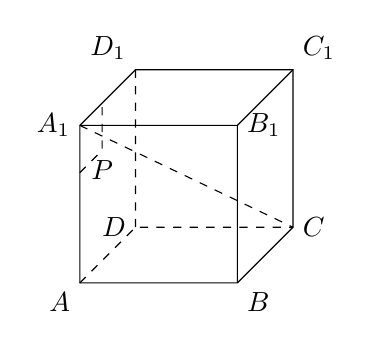
\begin{tikzpicture}
        \draw (0,0) node [below left] {$A$} coordinate (A) --++ (2,0) node [below right] {$B$} coordinate (B) --++ (45:{2/2}) node [right] {$C$} coordinate (C)
        --++ (0,2) node [above right] {$C_1$} coordinate (C1)
        --++ (-2,0) node [above left] {$D_1$} coordinate (D1) --++ (225:{2/2}) node [left] {$A_1$} coordinate (A1) -- cycle;
        \draw (A) ++ (2,2) node [right] {$B_1$} coordinate (B1) -- (B) (B1) --++ (45:{2/2}) (B1) --++ (-2,0);
        \draw [dashed] (A) --++ (45:{2/2}) node [left] {$D$} coordinate (D) --++ (2,0) (D) --++ (0,2);
        \draw [dashed] (A1) -- (C);
        \draw [dashed] (A1) ++ (0,-0.6) --++ (45:0.4) coordinate (P) --++ (0,0.6);
        \draw (P) node [below] {$P$};
    \end{tikzpicture}
\end{center}
\fourch{$ABCD$}{$BB_1C_1C$}{$CC_1D_1D$}{$AA_1B_1B$}
\item 命题$p$: 存在$a\in \mathbf{R}$且$a\ne 0$, 对任意的$x\in \mathbf{R}$, 均有$f(x+a)<f(x)+f(a)$恒成立. 已知命题$q_1$: $f(x)$单调递减, 且$f(x)>0$恒成立; 命题$q_2$: $f(x)$单调递增, 且存在${x_0}<0$使得$f({x_0})=0$. 则下列说法正确的是\bracket{20}.
\twoch{$q_1$、$q_2$都是$p$的充分条件}{只有$q_1$是$p$的充分条件}{只有$q_2$是$p$的充分条件}{$q_1$、$q_2$都不是$p$的充分条件}
\item 已知边长为$1$的正方形$ABCD$, 正方形$ABCD$绕$BC$旋转形成一个圆柱.\\
(1) 求圆柱的表面积;\\
(2) 正方形$ABCD$绕$BC$逆时针旋转$\dfrac{\pi}2$到$A_1BCD_1$, 求$AD_1$与平面$ABCD$所成的角.
\begin{center}
    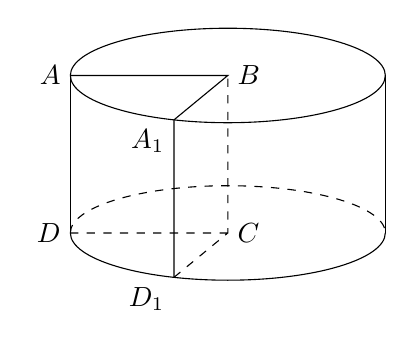
\begin{tikzpicture}
        \draw (-2,0) arc (180:360:2 and 0.6);
        \draw [dashed] (-2,0) arc (180:0:2 and 0.6);
        \draw (-2,2) arc (180:540:2 and 0.6);
        \draw (-2,2) node [left] {$A$} -- (0,2) node [right] {$B$} --++ ({2*cos(250)},{0.6*sin(250)}) node [below left] {$A_1$} --++ (0,-2) node [below left] {$D_1$} coordinate (D1);
        \draw [dashed] (D1) -- (0,0) node [right] {$C$} -- (0,2) (0,0) -- (-2,0) node [left] {$D$};
        \draw (-2,0) -- (-2,2) (2,0) -- (2,2);
    \end{tikzpicture}
\end{center}
\item 已知$f(x)=\sin\omega x$($\omega>0$).\\
(1) $f(x)$的周期是$4\pi$, 求$\omega$, 并求此时$f(x)=\dfrac12$的解集;\\
(2) 已知$\omega=1$, $g(x)=f^2(x)+\sqrt3f(-x)f(\dfrac{\pi}2-x)$, $x\in [0,\dfrac{\pi}4]$, 求$g(x)$的值域.
\item 在研究某市交通情况时, 道路密度是指该路段上一定时间内通过的车辆数除以时间, 车辆密度是该路段一定时间内通过的车辆数除以该路段的长度, 现定义交通流量为$v=\dfrac qx$, $x$为道路密度, $q$为车辆密度, $v=f(x)=\begin{cases} 100-135(\dfrac13)^{\frac{80}x}, & 0<x<40,  \\ -k(x-40)+85, & 40 \le x\le 80, \end{cases}$ $k>0$.\\
(1) 若交通流量$v>95$, 求道路密度$x$的取值范围; \\
(2) 若道路密度$x=80$时, 测得交通流量$v=50$, 求车辆密度$q$的最大值.
\item 双曲线$C_1:\dfrac{x^2}4-\dfrac{y^2}{b^2}=1$与圆$C_2:x^2+y^2=4+b^2 \ (b>0)$交于点$A(x_A,y_A)$(第一象限), 曲线$\Gamma$由所有在$C_1$或$C_2$上, 且满足$|x|>x_A$的点组成, $C_2$与$x$轴的左、右交点分别记作$F_1,F_2$.\\
(1) 若$x_A=\sqrt6$, 求$b$的值;\\
(2) 若$b=\sqrt5$, 点$P$在曲线$\Gamma$上, 且在第一象限, $|PF_1|=8$, 求$\angle F_1PF_2$;\\
(3) 点$D(0,\dfrac{b^2}2+2)$, 过该点的直线斜率为$-\dfrac b2$的$l$和$\Gamma$有且只有两个交点, 记作$M,N$, 用$b$表示$\overrightarrow{OM}\cdot \overrightarrow{ON}$, 并求$\overrightarrow{OM}\cdot \overrightarrow{ON}$的取值范围.
\item 已知有限数列$\{a_n\}$, 若满足$|a_1-a_2|\le |a_1-a_3|\le \cdots \le |a_1-a_m|$, $m$是项数, 则称$\{a_n\}$满足性质$P$.\\
(1) 判断数列$3,2,5,1$和$4,3,2,5,1$是否具有性质$P$, 请说明理由;\\
(2) 若首项$a_1=1$, 公比为$q$的等比数列, 项数为$10$, 具有性质$P$, 求$q$的取值范围;\\
(3) 若$\{a_n\}$是$1,2,\cdots,m$的一个排列($m\ge 4$), $\{b_n\}$符合$b_k=a_{k+1}$($k=1,2,\cdots,m-1$), $\{a_n\}$, $\{b_n\}$都具有性质$P$, 求所有满足条件的$\{a_n\}$.
\end{enumerate}

\newpage




{\bf 2019年秋考}

\begin{enumerate}[1.]
\item 已知集合$A=(-\infty,3)$, $B=(2,+\infty)$, 则$A\cap B=$\blank{50}.
\item 已知$z\in \mathbf{C}$. 若$\dfrac{1}{z-5}=\mathrm{i}$($\mathrm{i}$为虚数单位), 则$z=$\blank{50}.
\item 已知向量$\overrightarrow{a}=(1,0,2)$, $\overrightarrow{b}=(2,1,0)$, 则$\overrightarrow{a}$与$\overrightarrow{b}$的夹角为\blank{50}.
\item 在二项式$(2x+1)^5$的展开式中, $x^2$的系数是\blank{50}.
\item 已知$x,y$满足$\begin{cases} x\ge 0, \\ y \ge 0, \\ x+y \le 2,\end{cases}$ 则$2x-3y$的最小值为\blank{50}.
\item  已知函数$f(x)$的周期为$1$, 当$0<x\le 1$时, $f(x)=\log_2 x$, 则$f\left(\dfrac{3}{2}\right)$的值为\blank{50}.
\item 已知$x,y\in \mathbf{R}^*$, 且满足$\dfrac{1}{x}+2y=3$, 则$\dfrac{y}{x}$的最大值为\blank{50}.
\item 已知数列$\{a_n\}$的前$n$项和为$S_n$, 且满足$S_n+a_n=2$, 则$S_5=$\blank{50}.
\item 过曲线$y^2=4x$的焦点$F$并垂直于$x$轴的直线分别与曲线$y^2=4x$交于$A$、$B$, $A$在$B$的上方, $M$为抛物线上一点, $\overrightarrow{OM}=\lambda \overrightarrow{OA}+(\lambda-2) \overrightarrow{OB}$, 则$\lambda=$\blank{50}.
\item 某三位数密码, 每位数字可在$0$至$9$这$10$个数字中任选一个, 则该三位数密码中, 恰有两位数字相同的概率是\blank{50}.
\item 已知数列$\{a_n\}$满足$a_n<a_{n+1} \ (n\in \mathbf{N}^*)$, 若$P_n(n,a_n) \ (n\ge 3)$均在双曲线$\dfrac{x^2}{2}-\dfrac{y^2}{6}=1$上, 则$\displaystyle\lim_{n\to \infty}|P_nP_{n+1}|=$\blank{50}.
\item 已知$f(x)=\left|\dfrac{2}{x-1}-a\right| \ (x>1, \ a>0)$, $f(x)$的图像与$x$轴的交点为$A$, 若对于$f(x)$的图像上任意一点$P$, 在其图像上总存在另一点$Q$($P$、$Q$异于$A$), 满足$AP\perp AQ$, 且$|AP|=|AQ|$, 则$a=$\blank{50}.
\item 已知直线$l$的方程为$2x-y+c=0$, 则$l$的一个方向向量$\overrightarrow{d}$可以是\bracket{15}.
\fourch{$(2,-1)$}{$(2,1)$}{$(-1,2)$}{$(1,2)$}
\item 一个直角三角形的两直角边长分别为$1$和$2$, 将该三角形分别绕其两直角边所在直线旋转, 得到的两个圆锥的体积之比为\bracket{15}.
\fourch{$1$}{$2$}{$4$}{$8$}
\item 已知$\omega\in \mathbf{R}$, 函数$f(x)=(x-6)^2\cdot \sin (\omega x)$. 若存在常数$a\in \mathbf{R}$, 使得$f(x+a)$为偶函数, 则$\omega$的值可能为\bracket{15}.
\fourch{$\dfrac{\pi}{2}$}{$\dfrac{\pi}{3}$}{$\dfrac{\pi}{4}$}{$\dfrac{\pi}{5}$}
\item 已知$\tan\alpha\tan\beta=\tan(\alpha+\beta)$, 有下列两个结论: \textcircled{1} 存在$\alpha$在第一象限, $\beta$在第三象限; \textcircled{2} 存在$\alpha$在第二象限, $\beta$在第四象限; 则\bracket{15}.
\fourch{\textcircled{1}\textcircled{2}均正确}{\textcircled{1}\textcircled{2}均错误}{\textcircled{1}对\textcircled{2}错}{\textcircled{1}错\textcircled{2}对}
\item 如图, 在长方体$ABCD-A_1B_1C_1D_1$中, $M$为$BB_1$上一点, 已知$BM=2$, $CD=3$, $AD=4$, $AA_1=5$. \\
(1) 求直线$A_1C$与平面$ABCD{}$的夹角;\\
(2) 求点$A$到平面$A_1MC$的距离.
\begin{center}
    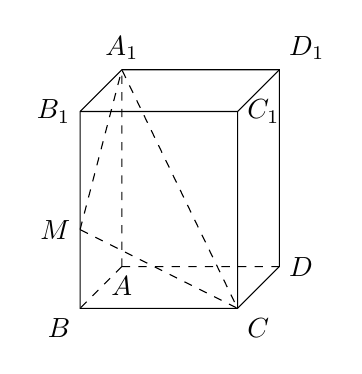
\begin{tikzpicture}[scale = 0.5]
        \draw [dashed] (0,0) coordinate (A) node [below] {$A$} -- (225:1.5) coordinate (B) node [below left] {$B$} (0,0) -- (4,0) coordinate (D) node [right] {$D$} (0,0) -- (0,5) coordinate (A1) node [above] {$A_1$};
        \draw (B) --++ (4,0) node [below right] {$C$} coordinate (C) -- (D) --++ (0,5) node [above right] {$D_1$} coordinate (D1) -- (A1) --++ (225:1.5) node [left] {$B_1$} coordinate (B1) -- cycle;
        \draw (D1) --++ (225:1.5) coordinate (C1) node [right] {$C_1$} (C1) -- (B1) (C) -- (C1);
        \draw [dashed] ($(B)!0.4!(B1)$) node [left] {$M$} -- (A1) -- (C) -- cycle; 
    \end{tikzpicture}
\end{center}
\item 已知$f(x)=ax+\dfrac{1}{x+1}, \ a\in \mathbf{R}$.\\
(1) 已知$a=1$时, 求不等式$f(x)+1<f(x+1)$的解集;\\
(2) 若$f(x)$在$x\in [1,2]$时有零点, 求$a$的取值范围.
\item 如图, $A-B-C$为海岸线, $AB$为线段, $\overset{\LARGE{\frown}}{BC}$为四分之一圆弧. $BD=39.2$km, $\angle BDC=22^\circ$, $\angle CBD=68^\circ$, $\angle BDA=58^\circ$.\\
(1) 求$\overset{\LARGE{\frown}}{BC}$的长度;\\
(2) 若$AB=40$km, 求$D$到海岸线$A-B-C$的最短距离(精确到$0.001$km).
\begin{center}
    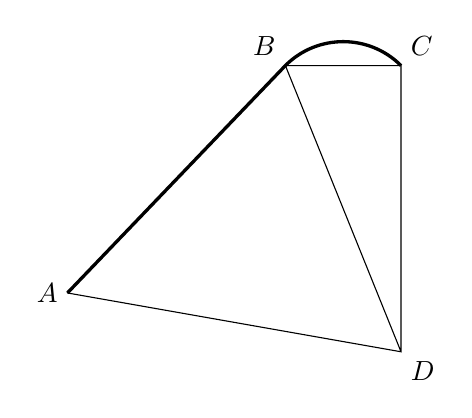
\begin{tikzpicture}
        \path (0,0) coordinate (D) node [below right] {$D$};
        \path (112:3.92) coordinate (B) node [above left] {$B$};
        \path (0,3.63456) coordinate (C) node [above right] {$C$};
        \path (-4.2365,0.747) coordinate (A) node [left] {$A$};
        \draw (D) -- (C) -- (B) (A) -- (D) -- (B);
        \draw [very thick] (C) arc (45:135:1.0383565) (A) -- (B);
    \end{tikzpicture}
\end{center}
\item 已知椭圆$\dfrac{x^2}{8}+\dfrac{y^2}{4}=1$, $F_1$、$F_2$为左、右焦点, 直线$l$过$F_2$, 交椭圆于$A$、$B$两点.\\
(1) 若直线$l$垂直于$x$轴, 求$|AB|$;
(2) 当$\angle F_1AB=90^\circ$, $A$在$x$轴上方时, 求$A$、$B$的坐标;
(3) 若直线$AF_1$交$y$轴于$M$, 直线$BF_1$交$y$轴于$N$, 是否存在直线$l$, 使得$S_{\triangle F_1AB}=S_{\triangle F_1MN}$? 若存在, 求出直线$l$的方程; 若不存在, 说明理由.
\item 数列$\{a_n\} \ (n=1,2,3,\cdots,100)$有$100$项, $a_1=a$, 且对任意$n=2,3,\cdots,100$, 存在$a_n=a_i+d, \ i=1,2,\cdots,n-1$. 若$a_k$与前$k-1$项中某一项相等, 则称$a_k$具有性质$P$.\\
(1) 若$a_1=1$, $d=2$, 求$a_4$的所有可能的值;\\
(2) 若$\{a_n\}$不是等差数列, 求证: 数列$\{a_n\}$中存在某些项具有性质$P$;\\
(3) 若$\{a_n\}$中恰有三项具有性质$P$, 这三项之和为$c$, 请用$a,d,c$表示$a_1+a_2+\cdots+a_{100}$.
\end{enumerate}

\newpage

{\bf 2018年秋考}

\begin{enumerate}[1.]
\item 行列式$\begin{vmatrix}
4 & 1 \\ 2 & 5
\end{vmatrix}$的值为\blank{50}.
\item 双曲线$\dfrac{x^2}{4}-y^2=1$的渐近线方程为\blank{50}.
\item 在$(1+x)^7$的二项展开式中, $x^2$项的系数为\blank{50}(结果用数值表示).
\item 设常数$a\in \mathbf{R}$, 函数$f(x)=\log_2(x+a)$. 若$f(x)$的反函数的图像经过点$(3,1)$, 则$a=$\blank{50}.
\item 已知复数$z$满足$(1+\mathrm{i})z=1-7\mathrm{i}$($\mathrm{i}$是虚数单位), 则$|z|=$\blank{50}.
\item 记等差数列$\{a_n\}$的前$n$项和为$S_n$. 若$a_3=0$, $a_6+a_7=14$, 则$S_7=$\blank{50}.
\item 已知$\alpha\in \left\{-2,-1,-\dfrac{1}{2},\dfrac{1}{2},1,2,3\right\}$. 若幂函数$f(x)=x^{\alpha}$为奇函数, 且在$(0,+\infty)$上递减, 则$\alpha=$\blank{50}.
\item 在平面直角坐标系中, 已知点$A(-1,0)$、$B(2,0)$, $E$、$F$是$y$轴上的两个动点, 且$|EF|=2$, 则$\overrightarrow{AE}\cdot \overrightarrow{BF}$的最小值为\blank{50}.
\item 有编号互不相同的五个砝码, 其中$5$克、$3$克、$1$克砝码各一个, $2$克砝码两个. 从中随机选取三个, 则这三个砝码的总质量为$9$克的概率是\blank{50}(结果用最简分数表示).
\item 设等比数列$\{a_n\}$的通项公式为$a_n=q^{n-1} \ (n\in \mathbf{N}^*)$, 前$n$项和为$S_n$. 若$\displaystyle\lim_{n\to \infty}\dfrac{S_n}{a_{n+1}}=\dfrac{1}{2}$, 则$q=$\blank{50}.
\item 已知常数$a>0$, 函数$f(x)=\dfrac{2^x}{2^x+ax}$的图像经过点$P\left(p,\dfrac{6}{5}\right)$, $Q\left(q,-\dfrac{1}{5}\right)$. 若$2^{p+q}=36pq$, 则$a=$\blank{50}.
\item 已知实数$x_1$、$x_2$、$y_1$、$y_2$满足: $x_1^2+y_1^2=1$, $x_2^2+y_2^2=1$, $x_1x_2+y_1y_2=\dfrac{1}{2}$, 则$\dfrac{|x_1+y_1-1|}{\sqrt{2}}+\dfrac{|x_2+y_2-1|}{\sqrt{2}}$的最大值为\blank{50}.
\item 设$P$是椭圆$\dfrac{x^2}{5}+\dfrac{y^2}{3}=1$上的动点, 则$P$到该椭圆的两个焦点的距离之和为\bracket{15}.
\fourch{$2\sqrt{2}$}{$2\sqrt{3}$}{$2\sqrt{5}$}{$4\sqrt{2}$}
\item 已知$a\in \mathbf{R}$, 则``$a>1$''是``$\dfrac{1}{a}<1$''的\bracket{15}.
\twoch{充分非必要条件}{必要非充分条件}{充要条件}{既非充分又非必要条件}
\item 《九章算术》中, 称底面为矩形而有一侧棱垂直于底面的四棱锥为阳马. 设$AA_1$是正六棱柱的一条侧棱, 如图. 若阳马以该正六棱柱的顶点为顶点、以$AA_1$为底面矩形的一边, 则这样的阳马的个数是\bracket{15}.
\begin{center}
    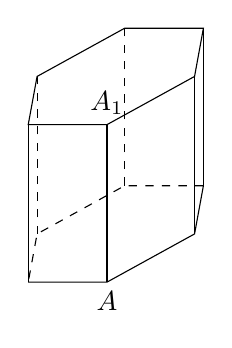
\begin{tikzpicture}
        \coordinate (A) at (0,0) node [below] {$A$};
        \path (A) --++ (45:{sqrt(3)/2}) --++ (0.5,0) coordinate (B);
        \path (A) --++ (45:{sqrt(3)}) coordinate (C);
        \path (C) --++ (-1,0) coordinate (D);
        \path (B) --++ (-2,0) coordinate (E);
        \coordinate (F) at (-1,0);
        \draw (F) -- (A) -- (B) -- (C);
        \draw [dashed] (C) -- (D) -- (E) -- (F);
        \foreach \i in {(A),(B),(C),(F)}{\draw \i --++ (0,2);};
        \foreach \i in {(D),(E)}{\draw [dashed] \i --++ (0,2);};
        \path (A) --++ (0,2) coordinate (A1) node [above] {$A_1$};
        \path (B) --++ (0,2) coordinate (B1);
        \path (C) --++ (0,2) coordinate (C1);
        \path (D) --++ (0,2) coordinate (D1);
        \path (E) --++ (0,2) coordinate (E1);
        \path (F) --++ (0,2) coordinate (F1);
        \draw (A1) -- (B1) -- (C1) -- (D1) -- (E1) -- (F1) -- cycle;
    \end{tikzpicture}
\end{center}
\fourch{$4$}{$8$}{$12$}{$16$}
\item 设$D$是含数$1$的有限实数集, $f(x)$是定义在$D$上的函数. 若$f(x)$的图像绕原点逆时针旋转$\dfrac{\pi}{6}$后与原图像重合, 则在以下各项中, $f(1)$的可能取值只能是\bracket{15}.
\fourch{$\sqrt{3}$}{$\dfrac{\sqrt{3}}{2}$}{$\dfrac{\sqrt{3}}{3}$}{$0$}
\item 已知圆锥的顶点为$P$, 底面圆心为$O$, 半径为$2$.\\
(1) 设圆锥的母线长为$4$, 求圆锥的体积;\\
(2) 设$PO=4$, $OA$、$OB$是底面半径, 且$\angle AOB=90^\circ$, $M$为线段$AB$的中点, 如图, 求异面直线$PM$与$OB$所成的角的大小.
\begin{center}
    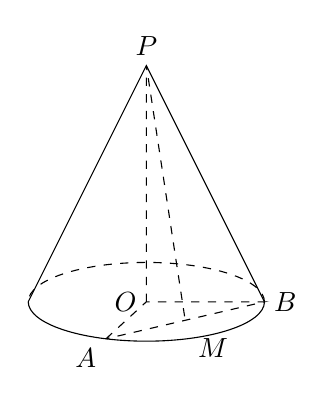
\begin{tikzpicture}
        \node (0,0) [left] {$O$} coordinate (O);
        \draw (-1.5,0) arc (180:360:1.5 and {1.5/3}) node [right] {$B$} coordinate (B);
        \draw [dashed] (1.5,0) arc (0:180:1.5 and {1.5/3}) coordinate (C);
        \draw (C) -- (0,3) node [above] {$P$} coordinate (P) -- (B); 
        \coordinate (A) at ({1.5*cos(250)},{0.5*sin(250)});
        \draw [dashed] (A)  node [below left] {$A$} -- (O) -- (B) -- cycle;
        \coordinate (M) at ($(A)!0.5!(B)$);
        \draw [dashed] (O) -- (P) -- (M) node [shift = {(-45:0.5)}] {$M$};
    \end{tikzpicture}
\end{center}
\item 设常数$a\in \mathbf{R}$, 函数$f(x)=a\sin 2x+2 \cos^2 x$.\\
(1) 若$f(x)$为偶函数, 求$a$的值;\\
(2) 若$f\left(\dfrac{\pi}{4}\right)=\sqrt{3}+1$, 求方程$f(x)=1-\sqrt{2}$在区间$[-\pi,\pi]$上的解.
\item 某群体的人均通勤时间, 是指单日内该群体中成员从居住地到工作地的平均用时. 某地上班族$S$中的成员仅以自驾或公交方式通勤. 分析显示: 当$S$中$x\% \ (0<x<100)$的成员自驾时, 自驾群体的人均通勤时间为
$$f(x)=\begin{cases}
30, & 0<x \le 30,\\ 2x+\dfrac{1800}{x}-90, & 30<x<100\end{cases} \ (\text{单位: 分钟}),$$
而公交群体的人均通勤时间不受$x$影响, 恒为$40$分钟. 试根据上述分析结果回答下列问题:\\
(1) 当$x$在什么范围内时, 公交群体的人均通勤时间少于自驾群体的人均通勤时间;\\
(2) 求该地上班族$S$的人均通勤时间$g(x)$的表达式; 讨论$g(x)$的单调性, 并说明其实际意义.
\item 设常数$t>2$. 在平面直角坐标系$xOy$中, 已知点$F(2,0)$, 直线$l:x=t$, 曲线$\Gamma:y^2=8x \ (0\le x\le t, \ y\ge 0)$. $l$与$x$轴交于点$A$、与$\Gamma$交于点$B$. $P$、$Q$分别是曲线$\Gamma$与线段$AB$上的动点.\\
(1) 用$t$表示点$B$到点$F$的距离;\\
(2) 设$t=3$, $|FQ|=2$, 线段$OQ$的中点在直线$FP$上, 求$\triangle AQP$的面积;\\
(3) 设$t=8$, 是否存在以$FP$、$FQ$为邻边的矩形$FPEQ$, 使得点$E$在$\Gamma$上? 若存在, 求点$P$的坐标; 若不存在, 说明理由.
\item 给定无穷数列$\{a_n\}$, 若无穷数列$\{b_n\}$满足: 对任意$n\in \mathbf{N}^*$, 都有$|b_n-a_n|\le 1$, 则称$\{b_n\}$与$\{a_n\}$``接近''.\\
(1) 设$\{a_n\}$是首项为$1$, 公比为$\dfrac{1}{2}$的等比数列, $b_n=a_{n+1}+1, \ n\in \mathbf{N}^*$. 判断数列$\{b_n\}$是否与$\{a_n\}$接近, 并说明理由;\\
(2) 设数列$\{a_n\}$的前四项为: $a_1=1$, $a_2=2$, $a_3=4$, $a_4=8$, $\{b_n\}$是一个与$\{a_n\}$接近的数列, 记集合$M=\{x|x=b_i, \ i=1,2,3,4\}$, 求$M$中元素的个数$m$;\\
(3) 已知$\{a_n\}$是公差为$d$的等差数列. 若存在数列$\{b_n\}$满足: $\{b_n\}$与$\{a_n\}$接近, 且在$b_2-b_1,b_3-b_2,\cdots,b_{201}-b_{200}$中至少有$100$个为正数, 求$d$的取值范围.
\end{enumerate}

\newpage

{\bf 2017年秋考}
\begin{enumerate}[1.]
\item 已知集合$A=\{1,2,3,4\}$, $B=\{3,4,5\}$, 则$A\cap B=$\blank{50}.
\item 若排列数$\mathrm{P}_6^m=6\times 5\times 4$, 则$m=$\blank{50}.
\item 不等式$\dfrac{x-1}{x}>1$的解集为\blank{50}.
\item 已知球的体积为$36\pi$, 则该球主视图的面积等于\blank{50}.
\item 已知复数$z$满足$z+\dfrac{3}{z}=0$, 则$|z|=$\blank{50}.
\item 设双曲线$\dfrac{x^2}{9}-\dfrac{y^2}{b^2}=1 \ (b>0)$的焦点为$F_1$、$F_2$, $P$为该双曲线上的一点, 若$|PF_1|=5$, 则$|PF_2|=$\blank{50}.
\item 如图, 以长方体$ABCD-A_1B_1C_1D_1$的顶点$D$为坐标原点, 过$D$的三条棱所在的直线为坐标轴, 建立空间直角坐标系. 若$\overrightarrow{DB_1}$的坐标为$(4,3,2)$, 则$\overrightarrow{AC_1}$的坐标是\blank{50}.
\begin{center}
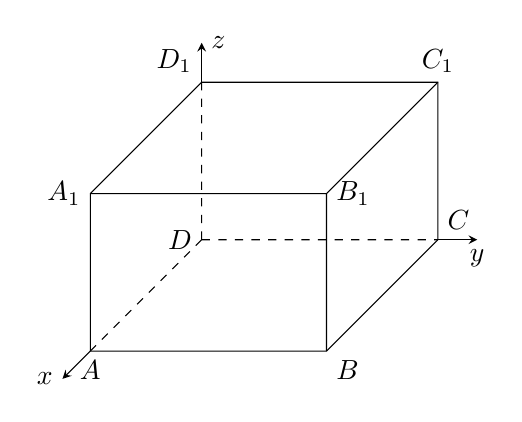
\begin{tikzpicture}[>=stealth]
\draw [dashed] (0,0) node [left] {$D$} -- (3,0) node [above right] {$C$} (0,0) -- (225:2) node [below] {$A$}  (0,0) -- (0,2) node [above left] {$D_1$};
\draw (3,0) -- (3,2) node [above] {$C_1$} -- (0,2) --++ (225:2) node [left] {$A_1$} --++ (0,-2) --++ (3,0) node [below right] {$B$} -- cycle;
\draw (0,2) ++ (225:2) --++ (3,0) node [right] {$B_1$} --+ (45:2) (3,0) ++ (225:2) --+ (0,2);
\draw [->] (3,0) -- (3.5,0) node [below] {$y$};
\draw [->] (0,2) -- (0,2.5) node [right] {$z$};
\draw [->] (225:2) -- (225:2.5) node [left] {$x$};
\end{tikzpicture}
\end{center}
\item 定义在$(0,+\infty)$上的函数$y=f(x)$的反函数为$y=f^{-1}(x)$. 若$g(x)=\begin{cases}3^x-1, & x\le 0,\\ f(x), & x>0\end{cases}$为奇函数, 则$f^{-1}(x)=2$的解为\blank{50}.
\item 已知四个函数: \textcircled{1} $y=-x$, \textcircled{2} $y=-\dfrac{1}{x}$, \textcircled{3} $y=x^3$, \textcircled{4} $y=x^{\frac{1}{2}}$. 从中任选$2$个, 则事件``所选$2$个函数的图像有且仅有一个公共点''的概率为\blank{50}.
\item 已知数列$\{a_n\}$和$\{b_n\}$, 其中$a_n=n^2, \ n\in \mathbf{N}^*$, $\{b_n\}$的项是互不相等的正整数. 若对于任意$n\in \mathbf{N}^*$, $\{b_n\}$的第$a_n$项等于$\{a_n\}$的第$b_n$项, 则$\dfrac{\lg (b_1b_4b_9b_{16})}{\lg(b_1b_2b_3b_4)}=$\blank{50}.
\item 设$\alpha_1,\alpha_2\in \mathbf{R}$, 且$\dfrac{1}{2+\sin\alpha_1}+\dfrac{1}{2+\sin(2\alpha_2)}=2$, 则$|10\pi-\alpha_1-\alpha_2|$的最小值等于\blank{50}.
\item 如图, 用$35$个单位正方形拼成一个矩形, 点$P_1,P_2,P_3,P_4$以及四个标记为``
\begin{tikzpicture}
\filldraw ({-0.0625*sqrt(3)},-0.0625) -- ({0.0625*sqrt(3)},-0.0625) -- (0,0.125) -- cycle;
\end{tikzpicture}''的点在正方形的顶点处, 设集合$\Omega=\{P_1,P_2,P_3,P_4\}$, 点$P\in \Omega$. 过$P$作直线$l_P$, 使得不在$l_P$上的``
\begin{tikzpicture}
\filldraw ({-0.0625*sqrt(3)},-0.0625) -- ({0.0625*sqrt(3)},-0.0625) -- (0,0.125) -- cycle;
\end{tikzpicture}''的点分布在$l_P$的两侧. 用$D_1(l_P)$和$D_2(l_P)$分别表示$l_P$一侧和另一侧的``
\begin{tikzpicture}
\filldraw ({-0.0625*sqrt(3)},-0.0625) -- ({0.0625*sqrt(3)},-0.0625) -- (0,0.125) -- cycle;
\end{tikzpicture}''的点到$l_P$的距离之和. 若过$P$的直线$l_P$中有且只有一条满足$D_1(l_P)=D_2(l_P)$, 则$\Omega$中所有这样的$P$为\blank{50}.
\begin{center}
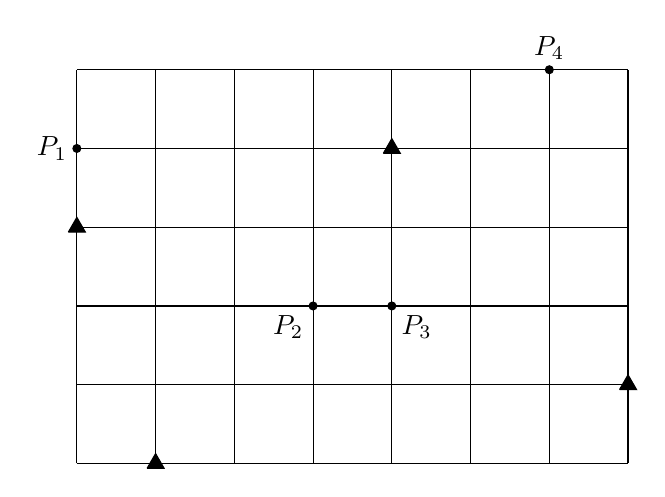
\begin{tikzpicture}
\foreach \i in {0,1,2,3,4,5,6,7}{\draw (\i,0) -- (\i,5);};
\foreach \i in {0,1,2,3,4,5}{\draw (0,\i) -- (7,\i);};
\filldraw  (1,0) ++ ({-0.0625*sqrt(3)},-0.0625) coordinate(P) --++ ({2*0.0625*sqrt(3)},0) --++ ({-0.0625*sqrt(3)},{3*0.0625}) -- (P);
\filldraw  (7,1) ++ ({-0.0625*sqrt(3)},-0.0625) coordinate(P) --++ ({2*0.0625*sqrt(3)},0) --++ ({-0.0625*sqrt(3)},{3*0.0625}) -- (P);
\filldraw  (0,3) ++ ({-0.0625*sqrt(3)},-0.0625) coordinate(P) --++ ({2*0.0625*sqrt(3)},0) --++ ({-0.0625*sqrt(3)},{3*0.0625}) -- (P);
\filldraw  (4,4) ++ ({-0.0625*sqrt(3)},-0.0625) coordinate(P) --++ ({2*0.0625*sqrt(3)},0) --++ ({-0.0625*sqrt(3)},{3*0.0625}) -- (P);
\filldraw (0,4) circle (0.05) node [left] {$P_1$};
\filldraw (3,2) circle (0.05) node [below left] {$P_2$};
\filldraw (4,2) circle (0.05) node [below right] {$P_3$};
\filldraw (6,5) circle (0.05) node [above] {$P_4$};
\end{tikzpicture}
\end{center}
\item 关于$x$、$y$的二元一次方程组$\begin{cases}
x+5y=0, \\ 2x+3y=4\end{cases}$的系数行列式$D$为\bracket{15}.
\fourch{$\begin{vmatrix}
0 & 5 \\ 4 & 3
\end{vmatrix}$}{$\begin{vmatrix}
1 & 0 \\ 2 & 4
\end{vmatrix}$}{$\begin{vmatrix}
1 & 5 \\ 2 & 3
\end{vmatrix}$}{$\begin{vmatrix}
6 & 0 \\ 5 & 4
\end{vmatrix}$}
\item 在数列$\{a_n\}$中, $a_n=\left(-\dfrac{1}{2}\right)^n, \ n\in \mathbf{N}^*$, 则$\displaystyle\lim_{n\to \infty}a_n$\bracket{15}.
\fourch{等于$-\dfrac{1}{2}$}{等于$0$}{等于$\dfrac{1}{2}$}{不存在}
\item 已知$a,b,c$为实常数, 数列$\{x_n\}$的通项$x_n=an^2+bn+c, \ n\in \mathbf{N}^*$, 则``存在$k\in \mathbf{N}^*$, 使得$x_{100+k},x_{200+k},x_{300+k}$成等差数列''的一个必要条件是\bracket{15}.
\fourch{$a\ge 0$}{$b\le 0$}{$c=0$}{$a-2b+c=0$}
\item 在平面直角坐标系$xOy$中, 已知椭圆$C_1:\dfrac{x^2}{36}+\dfrac{y^2}{4}=1$和$C_2:x^2+\dfrac{y^2}{9}=1$. $P$为$C_1$上的动点, $Q$为$C_2$上的动点, $w$是$\overrightarrow{OP}\cdot \overrightarrow{OQ}$的最大值. 记$\Omega=\{(P,Q)|P\text{在}C_1\text{上}, \ Q\text{在}C_2\text{上, 且}\overrightarrow{OP}\cdot \overrightarrow{OQ}=w\}$, 则$\Omega$中的元素有\bracket{15}.
\fourch{$2$个}{$4$个}{$8$个}{无穷个}
\item 如图, 直三棱柱$ABC-A_1B_1C_1$的底面为直角三角形, 两直角边$AB$和$AC$的长分别为$4$和$2$, 侧棱$AA_1$的长为$5$.\\
(1) 求三棱柱$ABC-A_1B_1C_1$的体积;\\
(2) 设$M$是$BC$中点, 求直线$A_1M$与平面$ABC$所成角的大小.
\begin{center}
\begin{tikzpicture}[scale=0.8]
    \draw (0,0) node [below right] {$A$} coordinate (A) -- (-4,0) node [left] {$B$} coordinate (B) (0,0) -- (45:1) node [right] {$C$} coordinate (C);
    \draw [dashed] (B) -- (C);
    \draw (A) --++ (0,5) node [right] {$A_1$} coordinate (A1) ;
    \draw (B) --++ (0,5) node [left] {$B_1$} coordinate (B1);
    \draw (C) --++ (0,5) node [above right] {$C_1$} coordinate (C1);
    \draw (A1) -- (B1) -- (C1) -- cycle;				
\end{tikzpicture}
\end{center}
\item 已知函数$f(x)=\cos^2 x-\sin^2 x+\dfrac{1}{2}, \ x\in (0,\pi)$.\\
(1) 求$f(x)$的单调递增区间;\\
(2) 设$\triangle ABC$为锐角三角形, 角$A$所对的边$a=\sqrt{19}$, 角$B$所对的边$b=5$, 若$f(A)=0$, 求$\triangle ABC$的面积.
\item 根据预测, 某地第$n \ (n\in \mathbf{N}^*)$个月共享单车的投放量和损失量分别为$a_n$和$b_n$(单位: 辆), 其中$a_n=\begin{cases}
5n^4+15, & 1\le n\le 3,\\ -10n+470, & n \ge 4,
\end{cases}$ $b_n=n+5$, 第$n$个月底的共享单车的保有量是前$n$个月的累计投放量与累计损失量的差.\\
(1) 求该地区第$4$个月底的共享单车的保有量;\\
(2) 已知该地共享单车停放点第$n$个月底的单车容纳量$S_n=-4(n-46)^2+8800$(单位: 辆). 设在某月底, 共享单车保有量达到最大, 问该保有量是否超出了此时停放点的单车容纳量?
\item 在平面直角坐标系$xOy$中, 已知椭圆$\Gamma: \dfrac{x^2}{4}+y^2=1$, $A$为$\Gamma$的上顶点, $P$为$\Gamma$上异于上、下顶点的动点. $M$为$x$正半轴上的动点.\\
(1) 若$P$在第一象限, 且$|OP|=\sqrt{2}$, 求$P$的坐标;\\
(2) 设$P\left(\dfrac{8}{5},\dfrac{3}{5}\right)$. 若以$A,P,M$为顶点的三角形是直角三角形, 求$M$的横坐标;\\
(3) 若$|MA|=|MP|$, 直线$AQ$与$\Gamma$交于另一点$C$, 且$\overrightarrow{AQ}=2\overrightarrow{AC}$, $\overrightarrow{PQ}=4\overrightarrow{PM}$, 求直线$AQ$的方程.
\item 设定义在$\mathbf{R}$上的函数$f(x)$满足: 对于任意的$x_1,x_2\in \mathbf{R}$, 当$x_1<x_2$时, 都有$f(x_1)\le f(x_2)$.\\
(1) 若$f(x)=ax^3+1$, 求$a$的取值范围;\\
(2) 若$f(x)$是周期函数, 证明: $f(x)$是常值函数;\\
(3) 设$f(x)$恒大于零. $g(x)$是定义在$\mathbf{R}$上的、恒大于零的周期函数, $M$是$g(x)$的最大值. 函数$h(x)=f(x)g(x)$. 证明: ``$h(x)$是周期函数''的充要条件是``$f(x)$是常值函数''.
\end{enumerate}

\end{document}

%一次测试